\chapter{Architecture Overview}

\section{Overview}

The feed handler will be designed so that as much code as possible is shared
between the standalone version and the dynamically linked library version.
In this implementation the standalone executable will just parse some arguments,
wrap them up into Q/K code and then pass this to the the library init function
to start the feed handler. The following figure shows which parts of the code
will be shared between the two different implementations.

 \begin{figure}[H]
 	\centering
 	\fbox{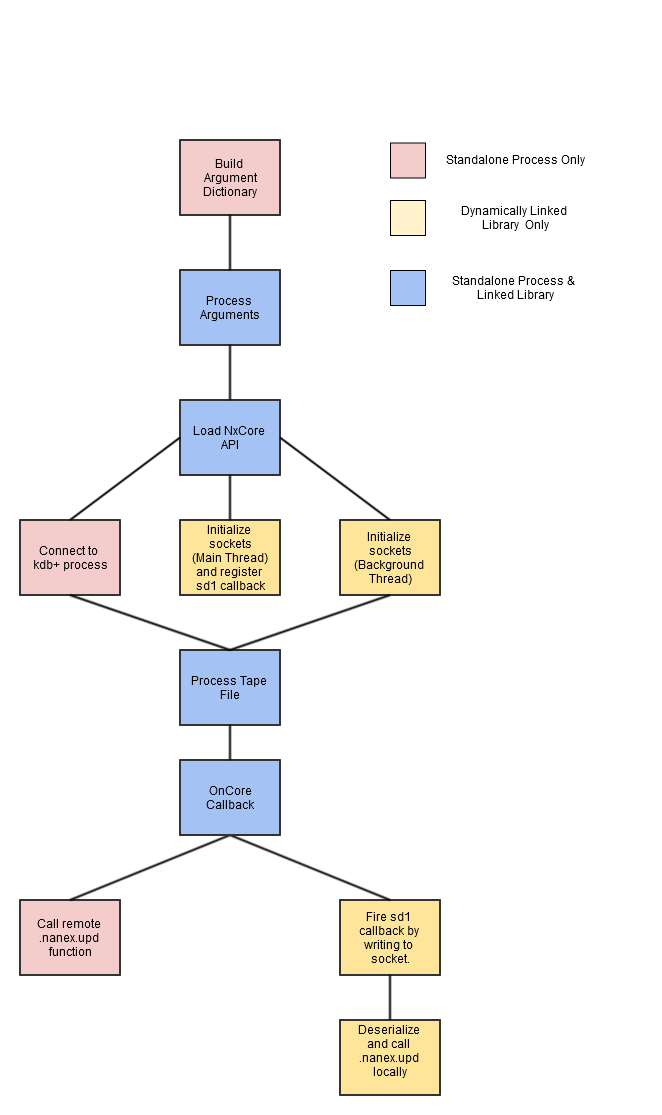
\includegraphics[scale=0.50]{figures/feedarchitecture.png}}
 	\caption{Feed Handler Architecture (both the Shared and Standalone components)}
 	\label{usingtheinputresourcepage}
 \end{figure}

The sections that are highlighted blue are parts of the code base that can be
shared between the two different types of feed handler. Most of the code that
performs the parsing of the data will be untouched, and the differences are
mostly in how the feeds are initialized.

For example, the standalone feed handler is expected to take its arguments
from the command line whilst the shared object version takes its arguments
as a dictionary passed to the initialization function. The standalone 
implementation can however re-use the shared objects code by converting it's
command line arguments into a K object that can then be passed to the 
shared object.

In order to keep as much code as possible identical between the two 
implementations, we will implement the standalone version of the feed handler
as a shell that just reads some arguments and then performs it's work via 
the shared library.

\section{Output Format}

There are some decisions that need to be made in terms of the output that the
feed handler will produce. Typically a q process will receive a list of atoms
which represent a row to be inserted into the database. The other type of update
that a q process will typically handle is a list of column vectors that represents
a batch of updates. The feed handler needs to convert a stream of serialized data
(e.g. binary/json/xml) into one of these structures before passing it to the receiving
process. Batching updates to a q process allows for more efficient IO operations
and less TCP/IP overhead. This in practice means that you will be trading off latency
for increased bandwidth.

 \begin{figure}[H]
 	\centering
 	\fbox{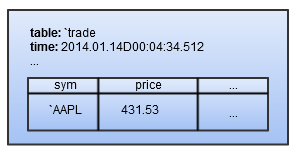
\includegraphics[scale=0.50]{figures/data_packet_format.png}}
 	\caption{Data packet format for the standalone feed handler}
 	\label{datapacketformat}
 \end{figure}

The feed handler will output messages in two different forms depending on how it is used.
In standalone mode, it will send K objects to the remote process. This allows the receiving
q process to decide which fields it wants to store in its tables without re-compiling the
feed handler.

When running the feed handler as a dynamically linked library, then we can take the dictionary
that is passed to the q process and unpack it before forwarding it onto the q process. This
method also allows us to easily add some filter operations before the data is forwarded.

In the provided implementation, this is defined as a .fh.upd function which takes the dictionary
data and performs some unpacking and automatic filling of data to match the schema. Through this
unpacking process we receive a list of atoms which are then pushed to the q process using the
.u.upd function. The dictionary data will be wrapped up inside another dictionary that contains
some meta data about the message, such as the time the message was sent and the table that it
should be pushed to.

This makes use of a \verb|.fh.tables| dictionary that just maps table names to the column names that
are present in that table. The example below shows how this could be implemented. Note that the
.fh.createrecord function will drop or fill data as appropriate and also reorder the columns to
fit the table schema.

\begin{figure}
\begin{lstlisting}
.fh.tp: .. // this is the handle to the q process
.fh.upd:{[x] .fh.tp(`.u.upd;.fh.createrecord[x`table;x`data]) }
.fh.createrecord:{[t;x] (.fh.tables[t],((cols[.fh.tables[t]] inter key[x])#x))}
\end{lstlisting}
\caption{Definitions of \textit{.fh.upd} and \textit{.fh.createrecord} that will unpack the dictionary structure}
\end{figure}

The alternative is to have the feed handler just push a list of atoms directly to the q process
which can provide a performance boost but at the cost of flexibility (the feed handler would
require compilation each time the schema is changed). This method means that the q process doesn't
need to be modified to handle special message types and the feed handler can just be pointed at other
kdb+ installs without any issues.

\section{Use of Background Threads}

As we will be running the feed handler as a shared library, it will need to
perform most of its work in a background thread so that the q processes is
still responsive. The standalone feed handler doesn't need a background thread
as it will just be running on its own, however to ensure we share as much code
as possible between the two implementations, we will start a background thread
and just wait/sleep in the main thread. It is also possible to have variations
on this architecture that use more threads to manage different feeds or to spread
the work of parsing across different instruments or asset classes for make better
use of multiple cores.

In the shared object implementation, the background thread will need to communicate
with the main q thread rather than an external q process. There are several possible
issues that can pop up related to memory management and concurrency that will be
explained later in the document. The solution suggested attempts to avoid concurrency
issues by having threads communicate with each other over a socket and minimizes the
amount of thought you will need to put into memory management by having each thread
only access K objects that it creates.

\section{Feed API}

In order to build the feed handler, we will need an example feed to work with.
We will build our own library that has a single function that allows us to
subscribe to the contents of the feed. No login or instrument subscription
logic will be included in the examples. The function that we use to listen for
new trades and quotes is called ProcessFeed.

\begin{figure}
\begin{lstlisting}[language=C]
/**
* ProcessFeed is a simple function that populates the statically allocated
* FeedData struct automatically and provides a pointer to it via a callback
* function for each message.
*/
void ProcessFeed(int (*) (const FeedData *));
\end{lstlisting}
\caption{The declaration of the callback function ProcessFeed}
\end{figure}

The function that is passed into ProcessFeed should expect to take a single parameter
which is a pointer to a FeedData struct (which holds the trade/quote data) and return
an integer which indicates if the feed should continue sending data.

The FeedData data structure is a tagged union. A member called \textbf{type} should
be checked before accessing the rest of the structure, otherwise you could be reading
from invalid data. For example, one you determine that the data received is trade data,
you can read the members in \textbf{data->core.*} (which are common to both trades and
quotes) and also the data in \textbf{data->msg.trade.*}.

The Feed itself is not intended to replicate a real feed in terms of the number of updates
received, or in ensuring that the trades and quotes pair off correctly. It is intended solely
to demonstrate connecting to a feed and serializing the data that is received.  The FeedData
structure is generated within the feed library itself and will be allocated in a static, shared
piece of memory. A reference to this structure will then be passed to the feed handler on each
callback (this is a common strategy in implementing these types of feeds).

The \verb|feed.so/feed.dll| will be built automatically alongside the code for the feed handler
itself, but as a separate object file. The feed itself has no dependencies and is platform
independent, so if you would like to use the feed for your own experiments, you should just copy
both the \verb|fakefeed.h| header file and the shared object into your own project.

\begin{figure}[h]
\begin{lstlisting}[language=C]
typedef struct _CoreMessage {
	char *sym;
	char *exg;
	int sequence;
	char cond[4];
} CoreMessage;

typedef struct _TradeMessage {
	int size;
	int volume;
	double price;
} TradeMessage;

typedef struct _QuoteMessage {
	int asksize;
	int bidsize;
	double askprice;
	double bidprice;
} QuoteMessage;

typedef struct _FeedData {
	int type;
	CoreMessage core;
	union {
		TradeMessage trade;
		QuoteMessage quote;
	} msg;
} FeedData;

\end{lstlisting}
\caption{The FeedData structure that is populated by the fake feed}
\end{figure}

The ProcessFeed function expects a constant \verb|FF_CONTINUE_FEED| to be returned if the feed should continue to process messages,
and \verb|FF_HALT_FEED| to be returned if not. These constants are defined in the \verb|fakefeed.h| header file.

\begin{figure}
\begin{lstlisting}[language=C]
int ExtractData(const FeedData *data)
{
	switch(data->type) {
		case FF_TRADE_MSG:
		// trade data can be accessed as in the examples below.
		//
		// data->core.sym;
		// data->msg.trade.size;
		break;
	case FF_QUOTE_MSG:
		// quote data can be accessed as in the examples below.
		//
		// data->core.sym;
		// data->msg.quote.askprice;
		break;
	}
	return FF_CONTINUE_FEED;
}

\end{lstlisting}
\caption{Example of processing messages from a feed in the callback}
\end{figure}

\section{Error Handling}

The error handling in the example code is kept to a minimum in order to keep the code simple, however in practice the
library code will need to be able to throw errors in both standalone and shared object formats. In order to handle errors
in this way, we need to use macro's to conditionally compile some parts of the code. The function should just print an
error to stderr when we are running as a standalone executable and then exit. For the shared library, we need to return
krr from our function so that it reaches the kdb+ process and raises a signal. This behaviour makes it easy for users to
respond to different types of errors in their q scripts without it just killing their process.

\begin{figure}
\begin{lstlisting}
////
// If called inside the standalone executable, this function will print the error to stderr and then exit
// immediately without attempting to release resources. If it is called from inside q as part of the DLL
// implementation it will just print an error message to the screen and then return.
//
K halt_on_error(const char *lngmsg, const char *kdbmsg)
{
#ifndef FEEDHANDLER_STANDALONE
	return krr(kdbmsg);
#elseif
	print_info(stderr, lngmsg);
	exit(EXIT_FAILURE);
	return (K) 0;
#endif
}
\end{lstlisting}
\caption{Definition of halt\_on\_error that will terminate in a standalone executable and raise a signal in a shared object}
\end{figure}

The function can then be used in the code by calling it and returning it's result to kdb+. 

\begin{figure}
\begin{lstlisting}
K init(K x) {
	if (!ProcessArgs(argv, argc)) {
		return halt_on_error("error: argument dictionary is invalid!", "badargs");
	}
}
\end{lstlisting}
\caption{Using the halt\_on\_error function to signal errors in init}
\end{figure}
